\documentclass[11pt,pdf,utf8,russian,aspectratio=169]{beamer}
\usepackage{cmap}
\usepackage[T2A]{fontenc}
\usepackage[english,russian]{babel}
\usepackage{subfig}
\usepackage{color}
\usepackage{multicol}
\usepackage{appendixnumberbeamer}
\usepackage{multicol}

\DeclareMathOperator*{\argmin}{arg\,min}

\DeclareMathOperator*{\argmax}{arg\,max}
%
% Choose how your presentation looks.
%
% For more themes, color themes and font themes, see:
% http://deic.uab.es/~iblanes/beamer_gallery/index_by_theme.html
%
\mode<presentation>
{
  \usetheme{Boadilla}      % or try Darmstadt, Madrid, Warsaw, ...
  \usecolortheme{seagull} % or try albatross, beaver, crane, ..

  \usefonttheme{structurebold}  % or try serif, structurebold, ...
  \setbeamertemplate{navigation symbols}{}
  \setbeamertemplate{caption}[numbered]
} 

/iffalse
1. Цель исследования
2. Постановка задач
3-5. Иллюстрации
6-7.Вар вывод
8. Теорема
9-10. Графики
11. Гиперпараметры
-14. Гиперпараметры
15-16. Результаты
17. Результаты
18. Список работ
/fi

\captionsetup[subfloat]{labelformat=empty}
\title[Оптимизация гиперпараметров моделей]{Градиентные методы оптимизации гиперпараметров моделей глубокого обучения}
\author{О.\,Ю.\,Бахтеев}
\institute[МФТИ]{Научный руководитель: д.ф.-м.н. В.В. Стрижов\\Московский Физико-Технический Институт (Государственный Университет)}     
%\institute[МФТИ]{Московский Физико-Технический Институт (Государственный Университет)}
\date[09.10.2017]{ММРО-2017 \\~\\09.10.2017}
\begin{document}

\begin{frame}
  \titlepage
\end{frame}

\begin{frame}{Цель работы}
\textbf{Исследуются}\\
Методы автоматического порождения и прореживания моделей глубокого обучения.

\textbf{Требуется}\\
Предложить алгоритм нахождения оптимальных значений гиперпараметров (параметров распределения параметров) модели.

\textbf{Проблемы нахождения оптимальных значений гиперпараметров}
\begin{itemize}
\item Многоэкстремальность задачи оптимизации параметров модели,
\item Вычислительная сложность оптимизации,
\item Большое количество гиперпараметров.
\end{itemize}

\textbf{Решение}\\
Предлагается оптимизировать параметры и гиперпараметры модели в единой процедуре с использованием градиентных методов. В качестве критерия оптимальности модели рассматривается нижняя оценка правдоподобия модели. 

\end{frame}


\begin{frame}                                                                                                                                   
\frametitle{Проблемы обучения сетей}                                                                                                            
Правдоподобие моделей с избыточным количеством параметров не меняется при удалении параметров.                                                       
\begin{figure}[h]                                                                                                                               
\centering                                                                                                                                      
\subfloat[Избыточность параметров модели]{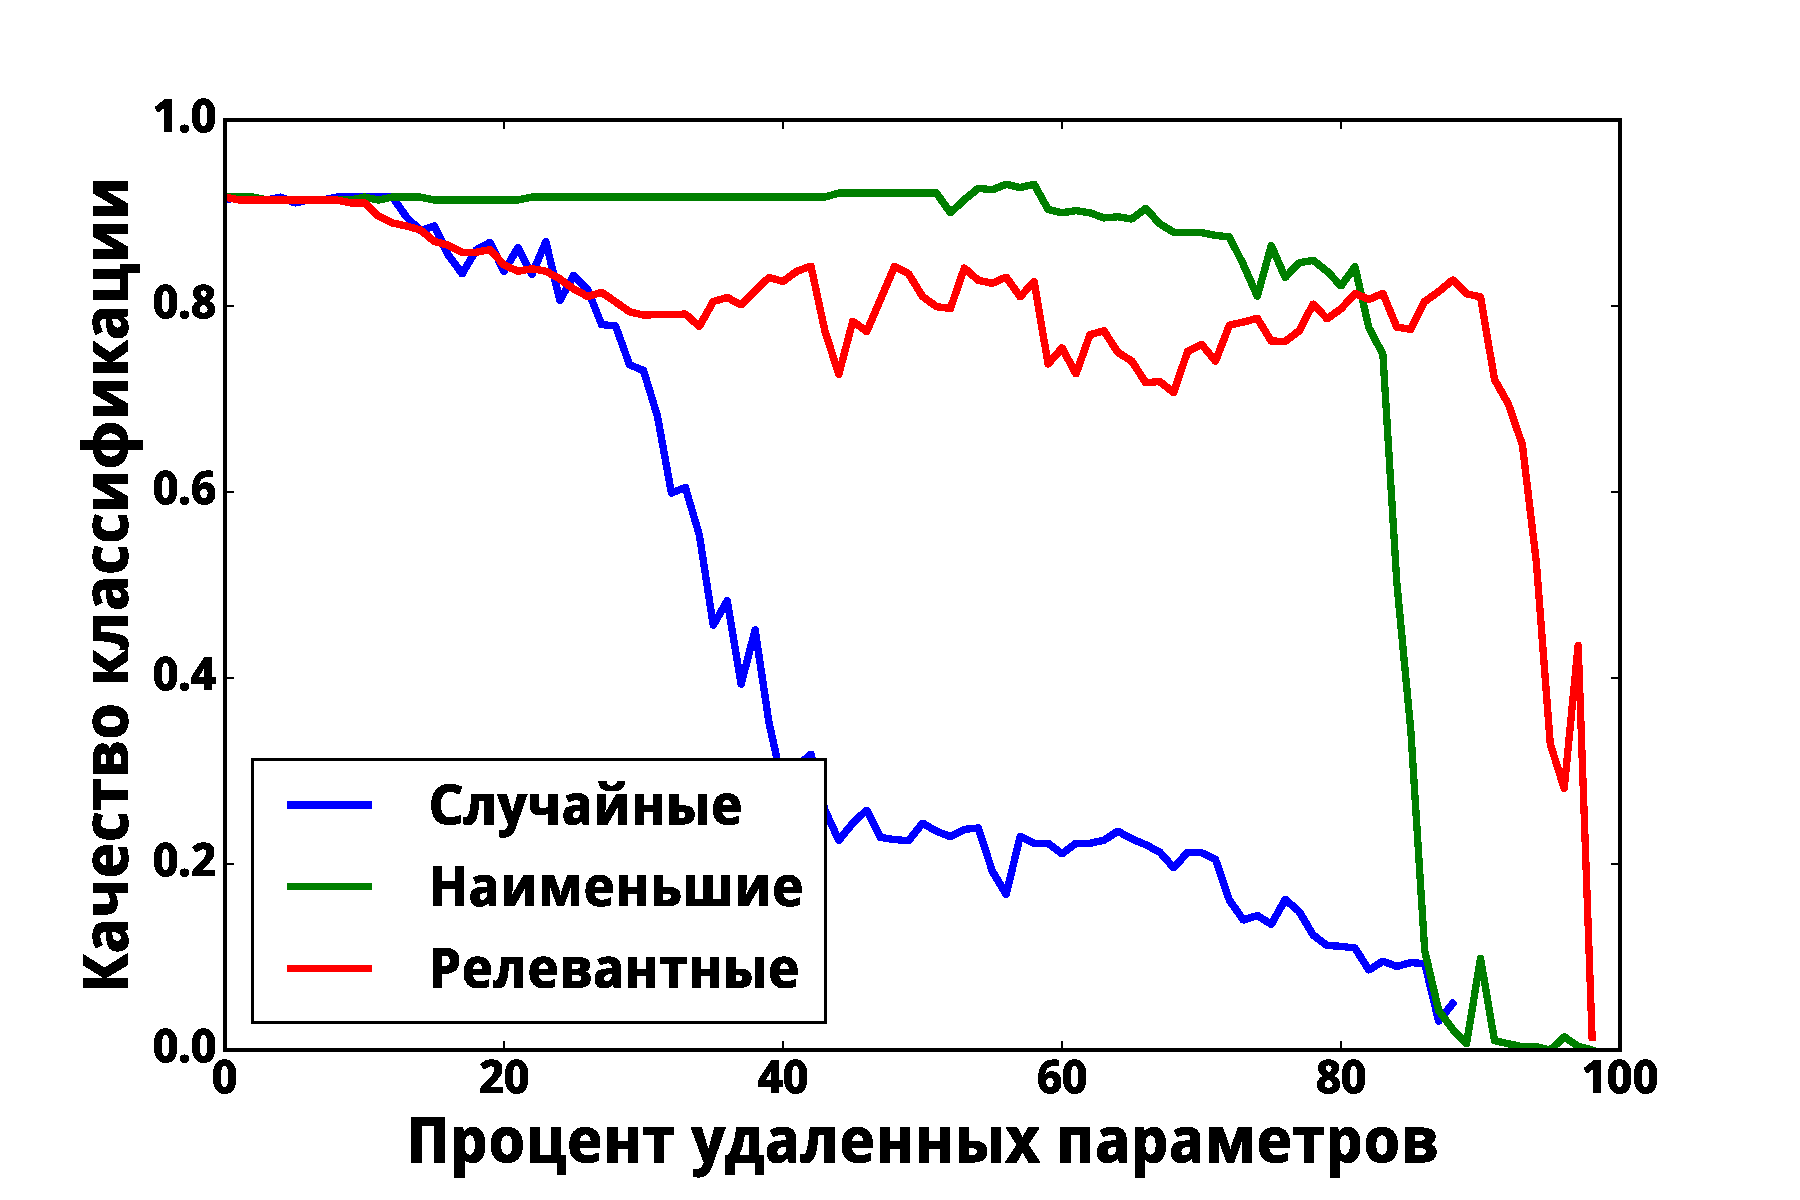
\includegraphics[width=0.45\textwidth]{./slide_plots/pruning.pdf}}                                          
\subfloat[Неустойчивость модели]{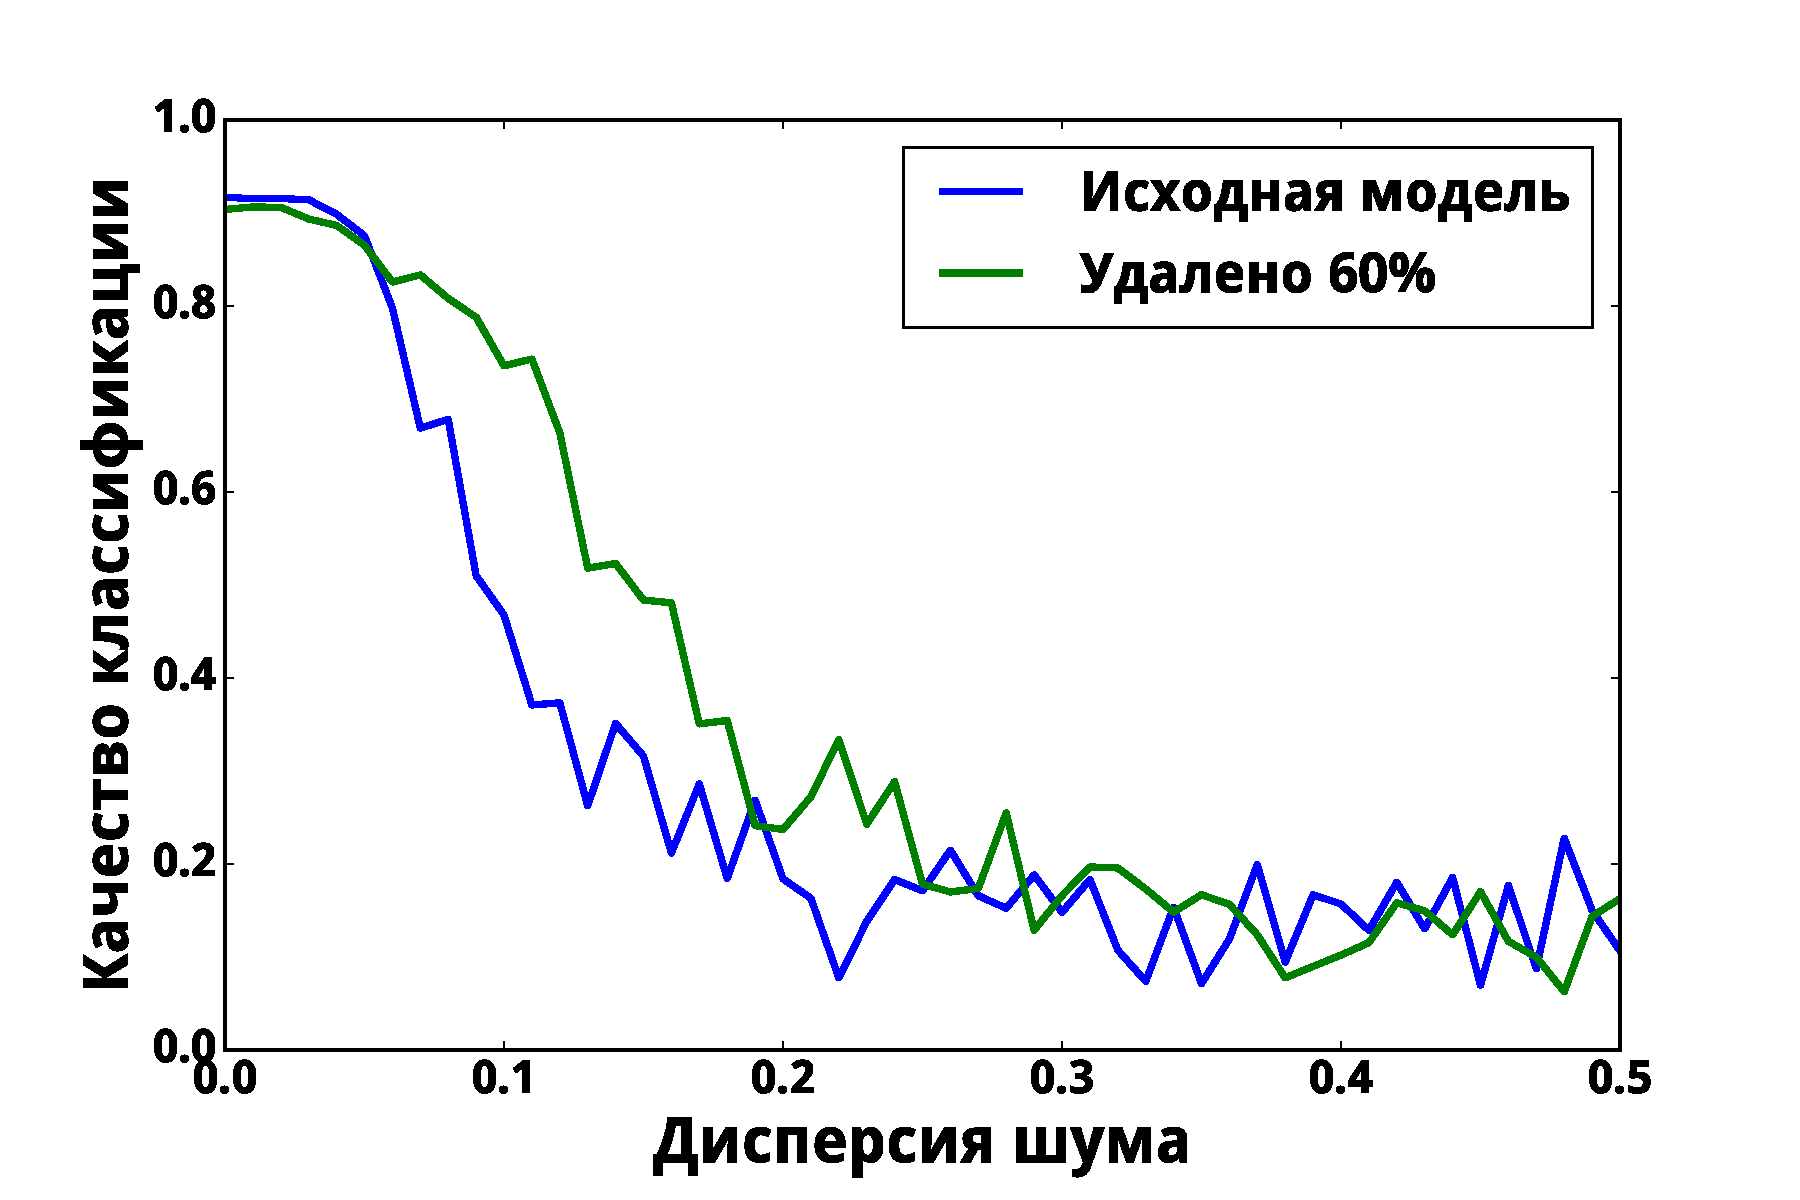
\includegraphics[width=0.45\textwidth]{./slide_plots/noise.pdf}}                                                     
\end{figure}                                                                                                                                    
                                                                                                                                                
\end{frame}    

\begin{frame}{Зависимость правдоподобия от гиперпараметров}
           
\begin{figure}[h]                                                                                                                               
\centering  
   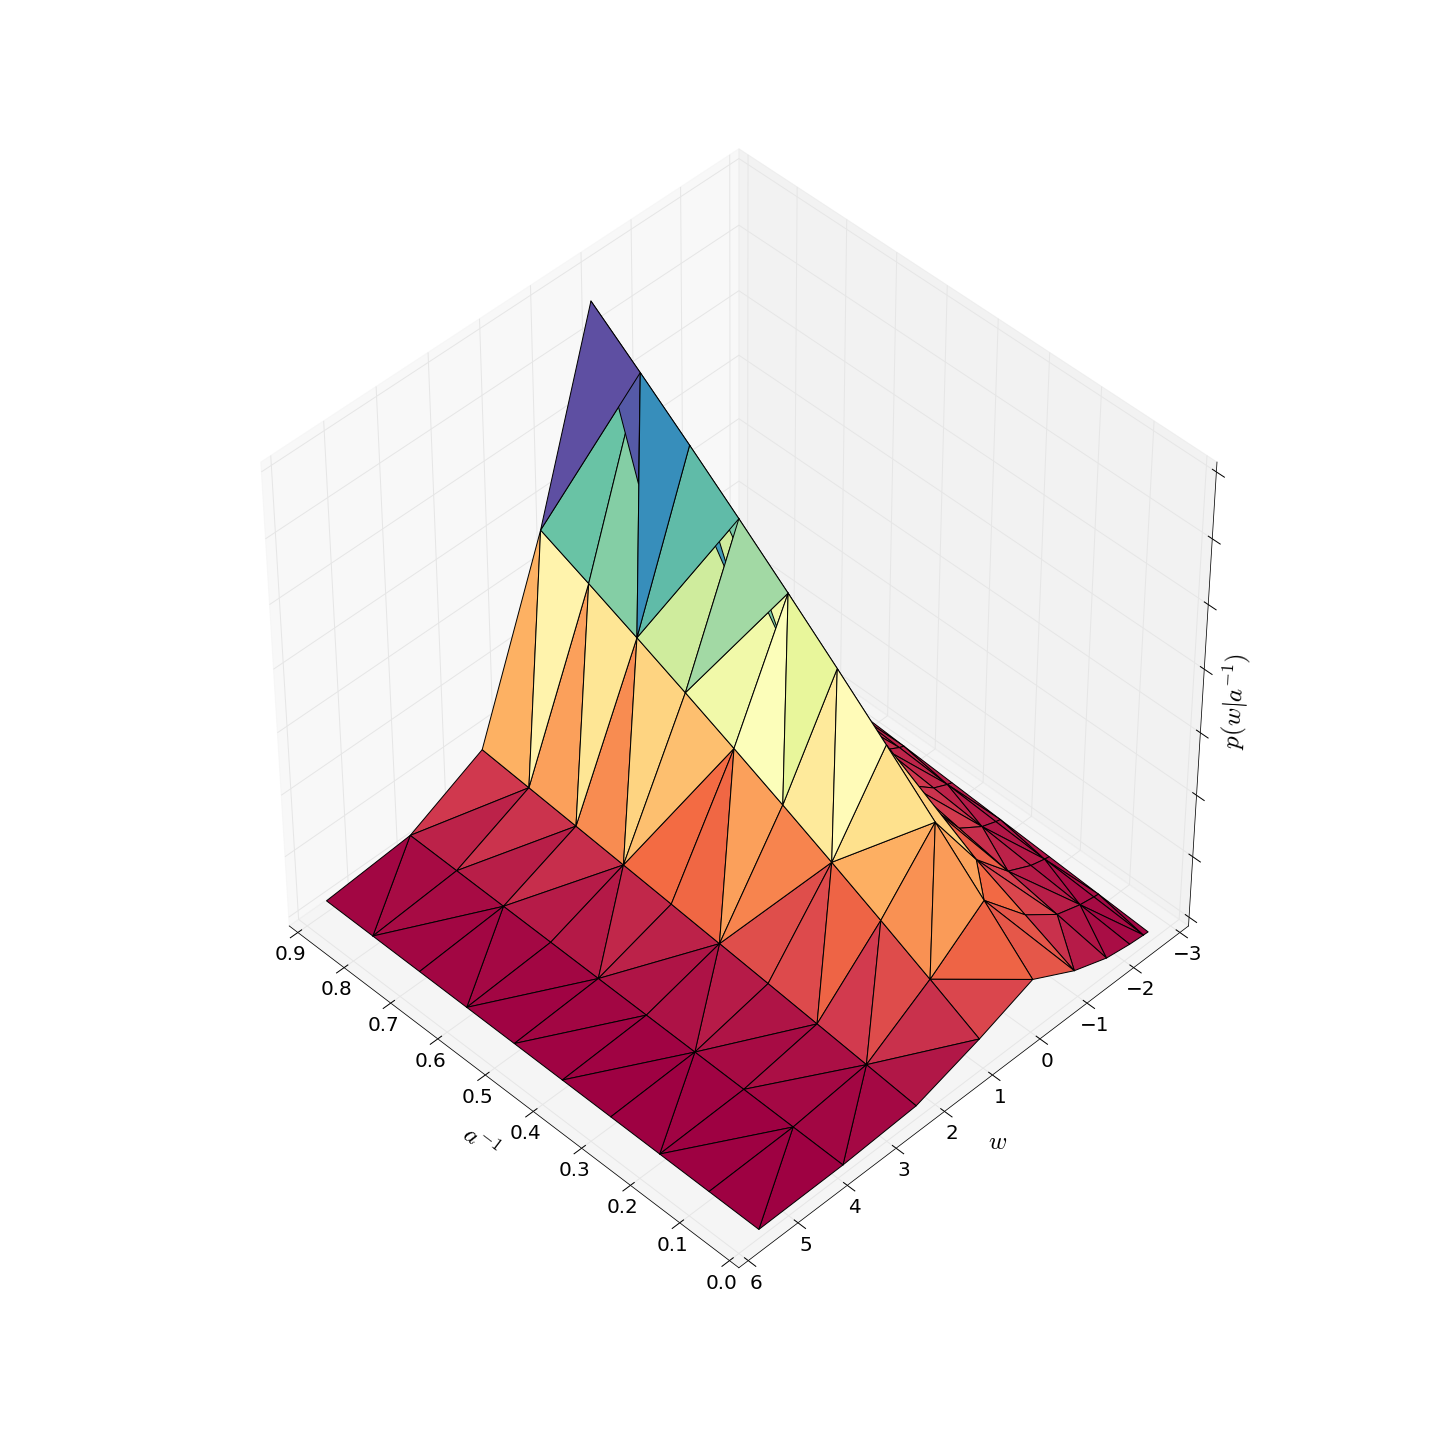
\includegraphics[width=0.75\textwidth]{./slide_plots/hyper.png}
\end{figure}
\end{frame}


\begin{frame}{Формальная постановка задачи}
Задана дифференцируемая по параметрам модель $\mathbf{f}(\mathbf{w}, \mathbf{x})$, задающая правдоподобие выборки $\textcolor{red}{p(\mathfrak{D}| \mathbf{w})}$.
Задано априорное распределение параметров модели:
\[
    \textcolor{blue}{p(\mathbf{w}|\mathbf{A}^{-1}) }\sim \mathcal{N}(\mathbf{0}, \mathbf{A}^{-1}) = \mathcal{N}(\mathbf{0}, \text{diag} [\alpha_1, \dots, \alpha_n]^\text{T}).
\]

Пусть $\boldsymbol{\theta}  \in \mathbb{R}^s$ --- множество параметров, подлежащих оптимизации (соответствует параметрам модели $\mathbf{w}$), \\
$L$ --- оптимизируемая функция потерь, \\$Q$ --- критерий качества модели.


Итоговая задача оптимизации:

\[
	\hat{\mathbf{A}}^{-1} = \argmax_{[\alpha_1, \dots, \alpha_n]^\text{T} \in \mathbb{R}^n} Q(\hat{\boldsymbol{\theta}}(\mathbf{A}^{-1}), \mathbf{A}^{-1}, \mathfrak{D}),
\]
\[
	\hat{\boldsymbol{\theta}}(\mathbf{A}^{-1}) =  \argmin_{\boldsymbol{\theta} \in \mathbb{R}^s} L(\boldsymbol{\theta}, \mathbf{A}^{-1}, \mathfrak{D}).
\]


\end{frame}

\iffalse
\begin{frame}{Формальная постановка задачи}
Задана выборка  \begin{equation}\label{eq:dataset}\mathfrak{D} = \{(\mathbf{x}_i,y_i)\}, i = 1,\dots,m,\end{equation} состоящая из множества пар <<объект-метка>>, $$\mathbf{x}_i \in \mathbf{X} \subset \mathbb{R}^n, \quad {y}_i \in \mathbf{y} \subset \mathbb{Y},$$ где $\mathbf{X}$ --- матрица объектов,  $\mathbf{y}$ --- вектор меток зависимой переменной $y$. 

Задана дифференцируемая по параметрам модель, приближающая зависимую переменную~$y$:
\[
	f:\mathbb{R}^n \to \mathbb{Y}, \quad \mathbf{w} \in \mathbb{R}^u.
\]

Модель $f$ задает правдоподобие выборки $p(\mathbf{y}|\mathbf{X}, \mathbf{w})$.
\end{frame}

\begin{frame}{Формальная постановка задачи}
Задано априорное распределение параметров модели:
\[
    p(\mathbf{w}|\mathbf{A}^{-1}) \sim \mathcal{N}(\mathbf{0}, \mathbf{A}^{-1}) = \mathcal{N}(\mathbf{0}, \text{diag} [\alpha_1, \dots, \alpha_n]^\text{T}).
\]

Пусть $\boldsymbol{\theta}  \in \mathbb{R}^s$ --- множество параметров, подлежащих оптимизации (соответствует параметрам модели $\mathbf{w}$).\\
Пусть $L$ --- оптимизируемая функция потерь, \\$Q$ --- критерий качества модели.


Итоговая задача оптимизации:

\[
	\hat{\mathbf{A}}^{-1} = \argmax_{[\alpha_1, \dots, \alpha_n]^\text{T} \in \mathbb{R}^n} Q(\hat{\boldsymbol{\theta}}(\mathbf{A}^{-1}), \mathbf{A}^{-1}, \mathfrak{D}),
\]
\[
	\hat{\boldsymbol{\theta}}(\mathbf{A}^{-1}) =  \argmin_{\boldsymbol{\theta} \in \mathbb{R}^s} L(\boldsymbol{\theta}, \mathbf{A}^{-1}, \mathfrak{D}).
\]


\end{frame}

\fi
\begin{frame}{L и Q: Кросс-валидация}
Разобьем выборку $\mathfrak{D}$ на $k$ равных частей:
\[
\mathfrak{D} = \mathfrak{D}_1 \sqcup \dots \sqcup \mathfrak{D}_k.
\]

Запустим $k$ оптимизаций модели, $r$-я модель обучается на выборках $\mathfrak{D}^r = \mathfrak{D}_1,\dots,\mathfrak{D}_{r-1},\mathfrak{D}_{r+1},\dots,\mathfrak{D}_k$.

Положим $\boldsymbol{\theta} = [\mathbf{w}_1, \dots, \mathbf{w}_k]$ --- параметры всех запусков модели.
\[
L(\boldsymbol{\theta}, \mathbf{A}^{-1}, \mathfrak{D}) = -\frac{1}{k}\sum_{r=1}^k \bigl(\frac{k}{k-1}\textcolor{blue}{\text{log}p(\mathfrak{D}^r|\mathbf{w}_r)} - \textcolor{red}{\text{log}p(\mathbf{w}_r|\mathbf{A}^{-1})}\bigr).
\]

\[
Q(\boldsymbol{\theta}, \mathbf{A}^{-1}, \mathfrak{D}) = \frac{1}{k}\sum_{r=1}^k k\textcolor{blue}{\text{log}p(\mathfrak{D}_r|\mathbf{w}_r)}.
\]


\end{frame}

\begin{frame}       
\begin{multicols}{2}
                                                                                                                            
\frametitle{Правдоподобие модели}                                                                                                         
                                                                                                                       
Модель $\mathbf{f} \in \mathfrak{F}$  оптимальна, если достигается максимум \textbf{правдоподобия модели}:                                      
\[                                                                                                                                              
        p(\mathfrak{D}|\mathbf{A}^{-1}) = \int_\mathbf{w} \textcolor{blue}{p( \mathfrak{D}| \mathbf{w})}\textcolor{red}{p(\mathbf{w}|\mathbf{A}^{-1})}d\mathbf{w}.                           
\]                                                                                                                                              
                                                                                                                                                
\begin{figure}[h]                                                                                                                               
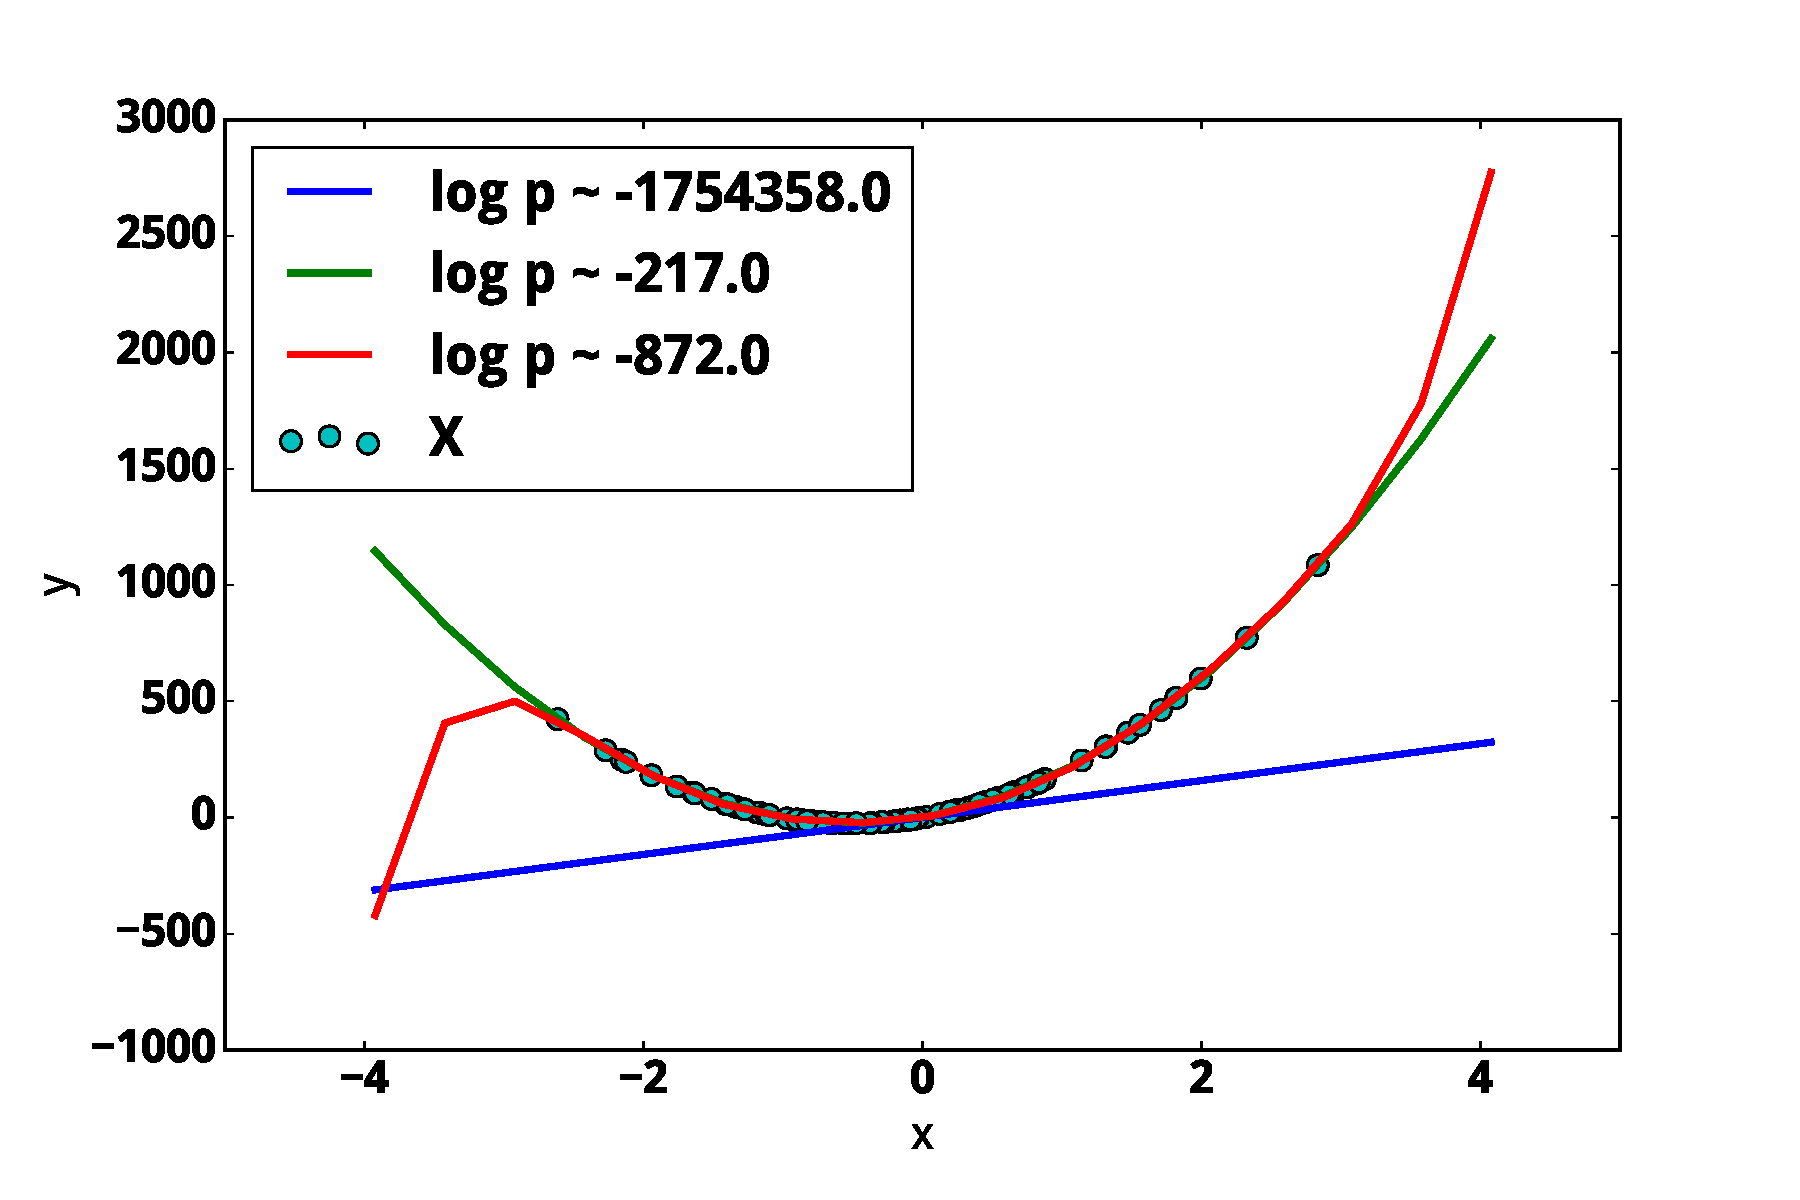
\includegraphics[width=0.45\textwidth]{./slide_plots/example.pdf}                                                                                      
\end{figure}                                                                                                                                    
\columnbreak
Пусть $q$ --- непрерывное распределение.
$$                                                                                                                                              
        \text{log}~p(\mathfrak{D}|\mathbf{A}^{-1}) \geq \int q(\mathbf{w})\text{log}~\frac{p(\mathfrak{D},\mathbf{w}|\mathbf{A}^{-1})}{q(\mathbf{w})}d\mathbf{w} =                                                                                                                                        
$$           
$$                                                                                                                                              
        = \textcolor{blue}{\int q(\mathbf{w})\text{log}~{p(\mathfrak{D} | \mathbf{w},\mathbf{A}^{-1})}d \mathbf{w}}  - \textcolor{red}{\text{D}_{\text{KL}}
} ,                                                                                                                                
$$      
где $$\textcolor{red}{\text{D}_{\text{KL}}} = -\int q(\mathbf{w})\text{log}~\frac{p(\mathbf{w} |\mathbf{A}^{-1})}{q(\mathbf{w})}d\mathbf{w}.$$ 

\end{multicols}
\end{frame}                                                                                                                                     
              
\begin{frame}
\frametitle{Вариационная оценка на основе мультистарта}
$$\text{log}p(\mathfrak{D}|\mathbf{A}) \geq \mathsf{E}_{q(\mathbf{w)}}[\text{log~}p (\mathfrak{D}, \mathbf{w}| \mathbf{A}^{-1})] - \mathsf{S}({q(\mathbf{w)}}),$$
$\mathsf{S}$ --- энтропия.

\textbf{Теорема [Бахтеев, 2016].}~Пусть $L$ --- функция потерь, градиент которой ---  непрерывно-дифференцируемая функция с константой Липшица $C$. Пусть $\boldsymbol{\theta} = [\mathbf{w}^1,\dots,\mathbf{w}^k]$ ---  начальные приближения оптимизации модели. Пусть $\gamma$ --- шаг градиентного спуска, такой что:
\begin{itemize}
\item $\gamma<\frac{1}{C}$,
\item $\gamma^{(-1)} > \max_{r \in \{1,\dots,k\}}\lambda_\text{max} (\mathbf{H}(\mathbf{w}^r))$.
\end{itemize}
Тогда
\small
\[
	\mathsf{S}(q^\tau(\mathbf{w})) -  \mathsf{S}(q^{\tau-1}(\mathbf{w}))  \sim  \frac{1}{k}\sum_{r=1}^k \bigl(\gamma Tr[\mathbf{H}(\mathbf{w}^r)] - \gamma^2 Tr[\mathbf{H}(\mathbf{w}^r)\mathbf{H}(\mathbf{w}^r)]  \bigr) + o_{\gamma \to 0}(1),
\]
где $\mathbf{H}$ --- гессиан функции потерь $L$, $q^\tau$ --- распределение $q(\mathbf{w})$ в момент оптимизации $\tau$.
\end{frame}


\begin{frame}
\frametitle{\smallВариационная оценка с использованием градиентного спуска}
Максимизация вариационной оценки эквивалентна минимизации $\text{D}_{\text{KL}}(q(\mathbf{w})||p(\mathbf{w} | \mathfrak{D},\mathbf{A}^{-1}))$.
Градиентный спуск не минимизирует $\text{D}_{\text{KL}}(q(\mathbf{w})||p(\mathbf{w} | \mathfrak{D},\mathbf{A}^{-1}))$.
\begin{multicols}{2}

\begin{figure}
\subfloat{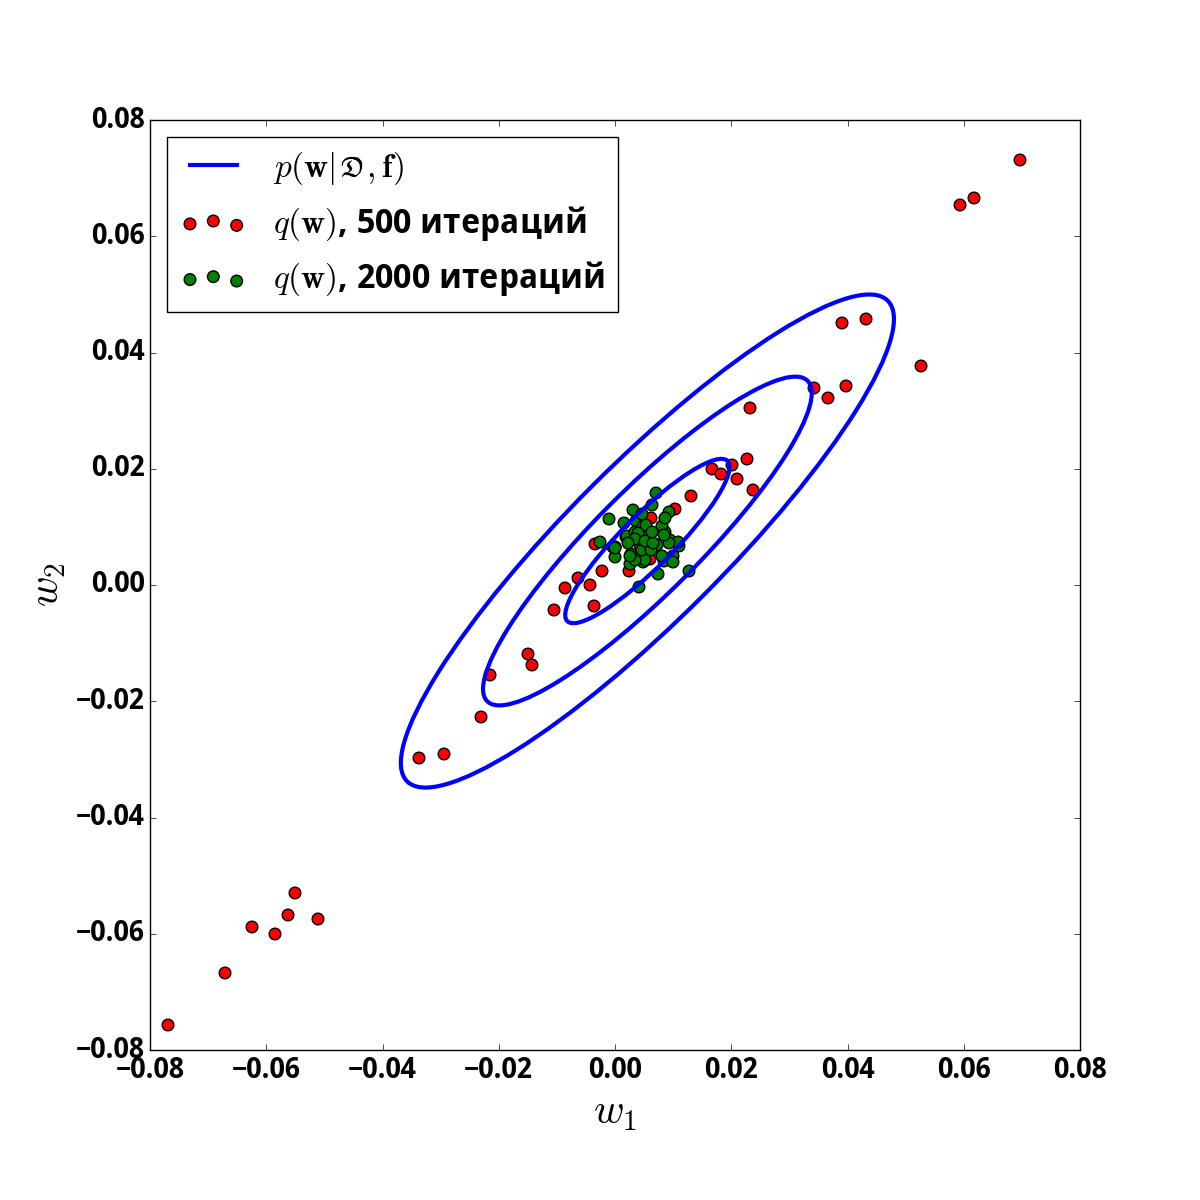
\includegraphics[width=0.42\textwidth]{./slide_plots/sgd_estimate.png}}
\end{figure}

\columnbreak


\begin{figure}
{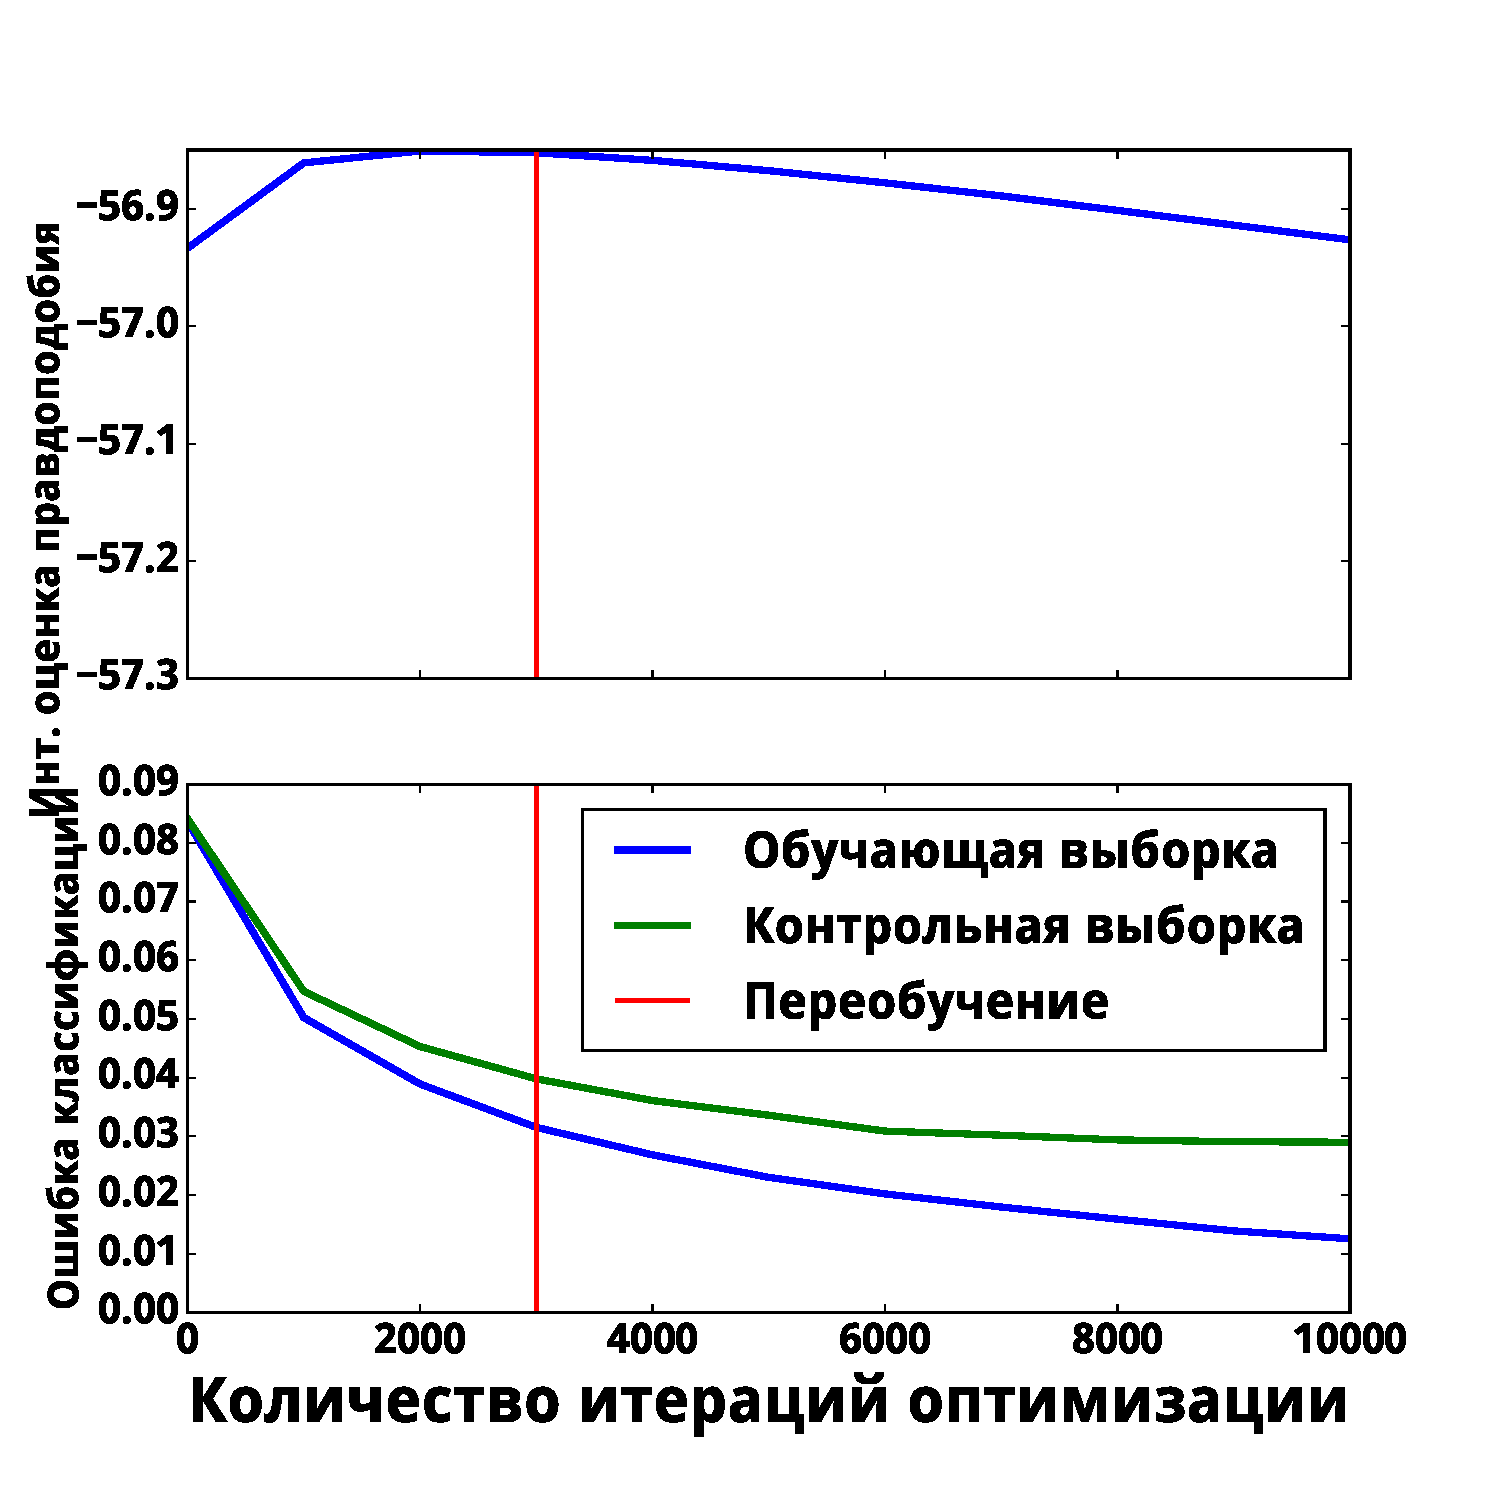
\includegraphics[width=0.42\textwidth]{./slide_plots/sgd_show.pdf}}
\end{figure}
\end{multicols}
\end{frame}

                                                                                                                                  
                                                                                                                                                
                                                                                                                                               
\iffalse                                                                                                                                                
\begin{frame}                                                                                                                                   
\frametitle{Вариационная оценка интегральной функции правдоподобия}                                                                             
\textbf{Проблема:} вычисление оценки правдоподобия модели имеет высокую вычислительную сложность.                                               
\small                                                                                                                                          
    
\textbf{Утверждение [Bishop, 2006].} Справедливы нижние оценки интегральной функции правдоподобия:                                              
$$                                                                                                                                              
        \text{log}~p(\mathfrak{D}|\mathbf{A}^{-1}) \geq \int q(\mathbf{w})\text{log}~\frac{p(\mathfrak{D},\mathbf{w}|\mathbf{A}^{-1})}{q(\mathbf{w})}d\mathbf{w} =                                                                                                                                        
$$           
$$                                                                                                                                              
        = -\text{D}_{\text{KL}} (q(\mathbf{w})||p(\mathbf{w}|\mathbf{A}^{-1})) + \int q(\mathbf{w})\text{log}~{p(\mathfrak{D} | \mathbf{w},\mathbf{A}^{-1}
)} d \mathbf{w},                                                                                                                                
$$      
где $$\text{D}_{\text{KL}}(q(\mathbf{w})||p(\mathbf{w} | \mathbf{A}^{-1})) = -\int q(\mathbf{w})\text{log}~\frac{p(\mathbf{w} |\mathbf{A}^{-1})}{q(\mathbf{w})}d\mathbf{w},$$ $q \in Q$ --- параметрическое семейство распределений.                                                                     
     

\end{frame} 
\fi           

\begin{frame}{L и Q: Вариационная оценка}
Пусть $q = \mathcal{N}(\boldsymbol{\mu}_q, \mathbf{A}^{-1}_q), \quad \boldsymbol{\theta} =  [\boldsymbol{\mu}_q, \mathbf{A}^{-1}_q].$ \\
Тогда вариационная оценка имеет вид:
$$
\textcolor{blue}{\int_{\mathbf{w}} q(\mathbf{w})\text{log}~{p(\mathfrak{D},\mathbf{w},\mathbf{A}^{-1})} d \mathbf{w}} - \textcolor{red}{D_\text{KL}\bigl(q (\mathbf{w} )|| p (\mathbf{w}|\mathbf{A}^{-1})\bigr)} \simeq
$$
$$
\sum_{i=1}^m \textcolor{blue}{\text{log}~p(\mathbf{x}_i | \mathbf{w}_i)} - \textcolor{red}{D_\text{KL}\bigl(q (\mathbf{w} )|| p (\mathbf{w}|\mathbf{A}^{-1})\bigr)} = -L(\boldsymbol{\theta}, \mathbf{A}^{-1}, \mathfrak{D}) = Q(\boldsymbol{\theta}, \mathbf{A}^{-1}, \mathfrak{D}),
$$
где $\mathbf{w}_i \sim q$.

Дивергенция $\textcolor{red}{D_\text{KL}\bigl(q (\mathbf{w} )|| p (\mathbf{w}|\mathbf{A}^{-1})\bigr)}$ вычисляется аналитически:
$$
\textcolor{red}{D_\text{KL}\bigl(q (\mathbf{w}) || p (\mathbf{w}|\mathbf{A}^{-1})\bigr)} = \frac{1}{2} \bigl( \text{tr} (\mathbf{A}\mathbf{A}^{-1}_q) + \boldsymbol{\mu}_q^\text{T}\mathbf{A}\boldsymbol{\mu}_q - n +\text{ln}~|\mathbf{A}^{-1}| - \text{ln}~|\mathbf{A}^{-1}_q| \bigr).
$$


\end{frame}

\begin{frame}{Общая схема алгоритма оптимизации}
\textbf{Вход:} количество итераций оптимизации гиперпараметров $\ell$, количество итераций оптимизации параметров $\tau$, 
длина шага градиентного спуска $\gamma$.

\begin{enumerate}
\item Повторять в цикле от $1,\dots, \ell$:
\begin{enumerate}
\item Инициализировать параметры $\boldsymbol{\theta}_0$.
\item Провести оптимизацию параметров с использованием стохастического градиентного спуска:
\[
    \hat{\boldsymbol{\theta}} = T \circ T \circ \dots \circ T(\boldsymbol{\theta}_0) = T^\tau(\boldsymbol{\theta}_0),
\]
где 
\[
    T(\boldsymbol{\theta}) =\boldsymbol{\theta} - \gamma \nabla_{\boldsymbol{\theta}} L(\boldsymbol{\theta}, \mathbf{A}^{-1}, \hat{\mathfrak{D}}),
\]
$\mathfrak{D}$ --- случайная подвыборка $\mathfrak{D}$.
\item Провести оптимизацию гиперпараметров: $Q(\hat{\boldsymbol{\theta}}(\mathbf{A}^{-1}), \mathbf{A}^{-1}, \mathfrak{D}) \to \max$.

\end{enumerate}
\end{enumerate}
\end{frame}

\begin{frame}{HOAG и Жадный алгоритм}
\begin{multicols}{2}
\begin{figure}[h]
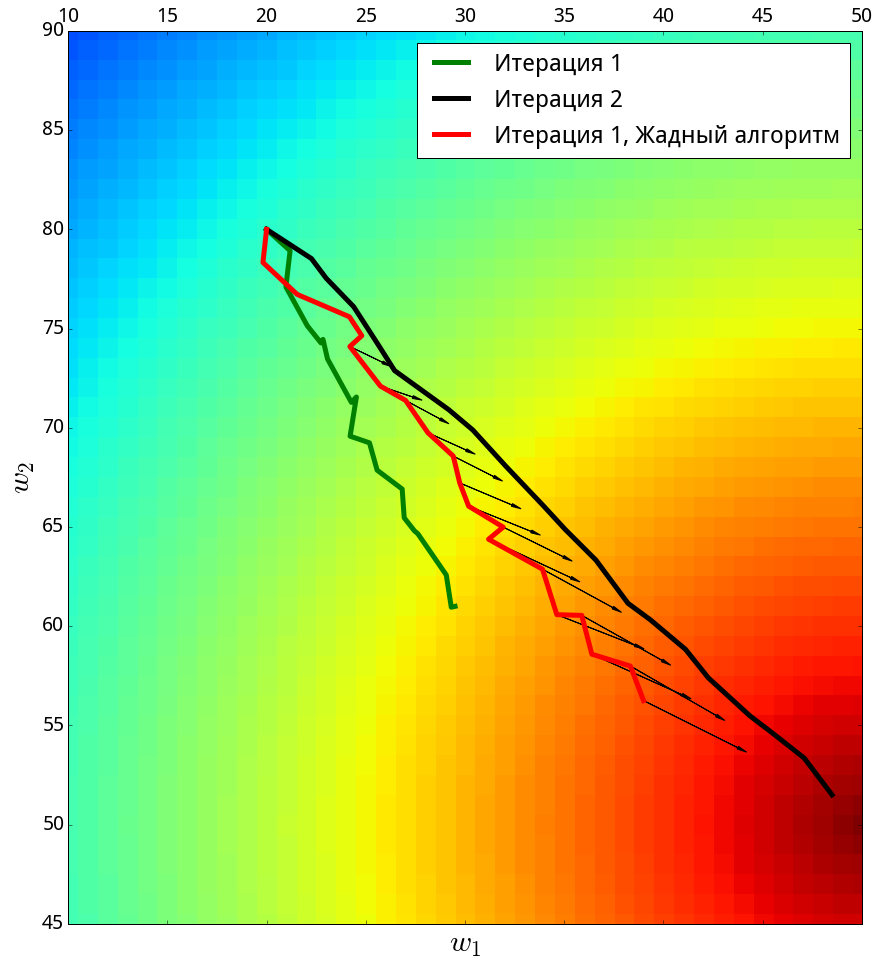
\includegraphics[width=0.45\textwidth]{./slide_plots/greed_hoag.png}
\end{figure}
\columnbreak
\textbf{Жадный алгоритм}
\[
	\mathbf{A}'^{-1} = \mathbf{A}^{-1} - \gamma_{\mathbf{A}} (\nabla_{\mathbf{A}^{-1}}  Q (T(\boldsymbol{\theta}) , \mathbf{A}^{-1}, \mathfrak{D})), %=  \mathbf{A}^{-1} - \gamma_{\mathbf{A}} (\nabla_{\mathbf{A}^{-1}}  Q(\boldsymbol{\theta} - \gamma \nabla L(\boldsymbol{\theta}, \mathbf{A}^{-1}), \mathbf{A}^{-1}, \mathfrak{D})),
\]
где $\gamma_{\mathbf{A}}$ --- длина шага оптимизации гиперпараметров.
\\~\\
\textbf{HOAG}
\[
\mathbf{A}'^{-1} = \mathbf{A}^{-1} - \gamma_{\mathbf{A}} \hat{\nabla}_{\mathbf{A}^{-1}} Q(T^\tau(\boldsymbol{\theta}_0),  \mathbf{A}^{-1}, \mathfrak{D})),
\]
где $\hat{\nabla}_{\mathbf{A}^{-1}}$ --- численное приближение градиента:
\[
%{\nabla}_{\mathbf{A}^{-1}} Q(T^\tau(\boldsymbol{\theta}_0), \mathbf{A}^{-1}, \mathfrak{D})) = 
\nabla_{\mathbf{A}^{-1}} Q(\hat{\boldsymbol{\theta}}) - (\frac{\partial^2{L}}{\partial \boldsymbol{\theta} \partial \mathbf{A}^{-1}})^\text{T} \mathbf{H}(L({\boldsymbol{\theta}}))^{-1} \nabla_{\boldsymbol{\theta}} Q.
\]
где $\mathbf{H}$ --- гессиан.
\end{multicols}
\end{frame}

\begin{frame}{Алгоритм DrMad}
\begin{multicols}{2}
\begin{figure}[h]
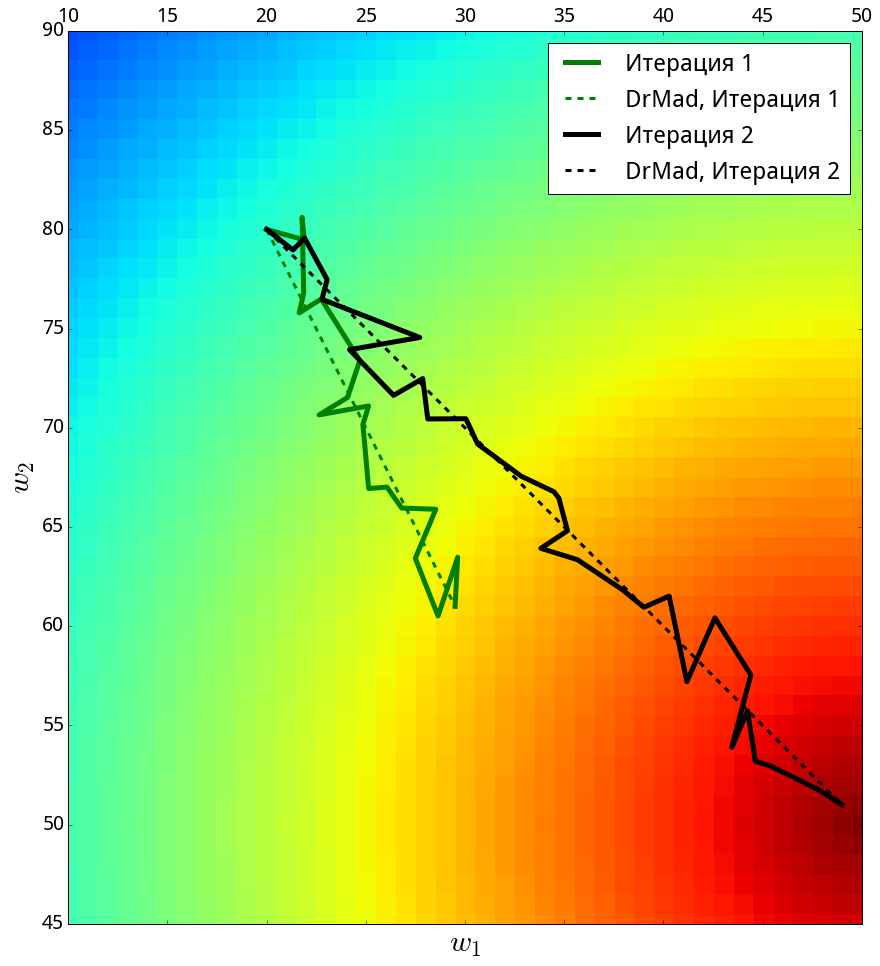
\includegraphics[width=0.45\textwidth]{./slide_plots/mad.png}
\end{figure}


Рассматривается оптимизация функции $Q(T^\tau(\boldsymbol{\theta}_0) , \mathbf{A}^{-1}, \mathfrak{D}))$ по \textbf{всей} истории оптимизации параметров.\\~\\
Вводятся предположения о линейности траектории оптимизации параметров. \\

Градиент $\nabla_\mathbf{A}^{-1} Q$ аккумулируется по правилу:
$$\nabla_{\mathbf{A}^{-1}} Q= \nabla_{\mathbf{A}^{-1}} Q - \gamma \nabla_{\boldsymbol{\theta}} Q(\boldsymbol{\theta}^\tau) \nabla_{\mathbf{A}^{-1}}  \nabla_{\boldsymbol{\theta}} L(\boldsymbol{\theta}^\tau).
$$
\end{multicols}

\end{frame}

\begin{frame}{Вычислительный эксперимент}
\textbf{Цель эксперимента:} анализ рассматриваемых алгоритмов и итоговых моделей.

\textbf{Данные:}
\begin{itemize}
\item Синтетические данные: 40 точек на плоскости. Модель: полином 12 степени.
\item Набор записей акселерометра WISDM. Рассматривается задача регрессии с нейронной сетью с одним скрытым слоем (10 нейронов).
\item Набор рукописных цифр MNIST. Рассматривается задача регрессии с нейронной сетью с одним скрытым слоем (300 нейронов).
\end{itemize}

В качестве Q и L рассматривается кросс-валидация ($k=4$) и вариационная оценка.
\end{frame}

\begin{frame}{Синтетические данные: результат}
\begin{multicols}{2}
\begin{figure}[h]
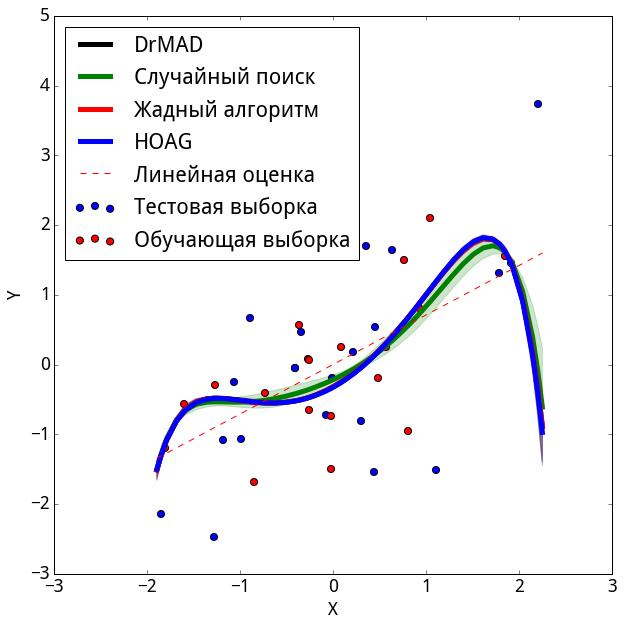
\includegraphics[width=0.4\textwidth]{./slide_plots/poly_cv.png}
\caption*{Кросс-Валидация}
\end{figure}

\begin{figure}[h]
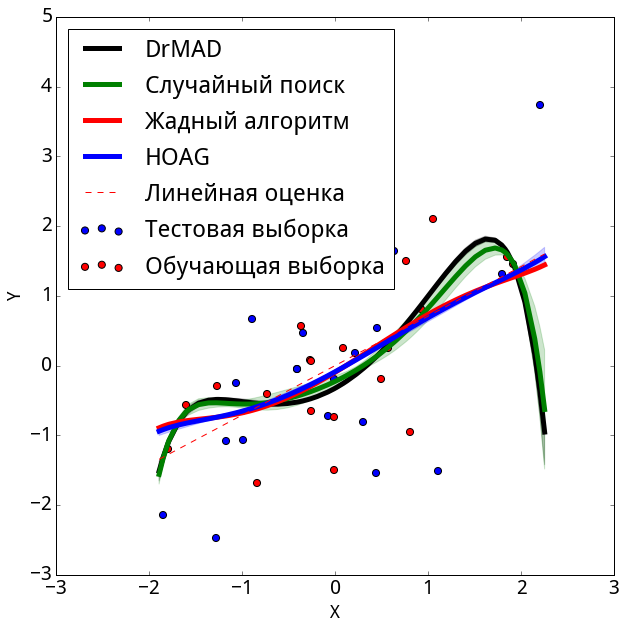
\includegraphics[width=0.4\textwidth]{./slide_plots/poly_var.png}
\caption*{Вариационная оценка}
\end{figure}
\end{multicols}

\end{frame}


\begin{frame}{WISDM: кросс-валидация}
\begin{figure}[h]
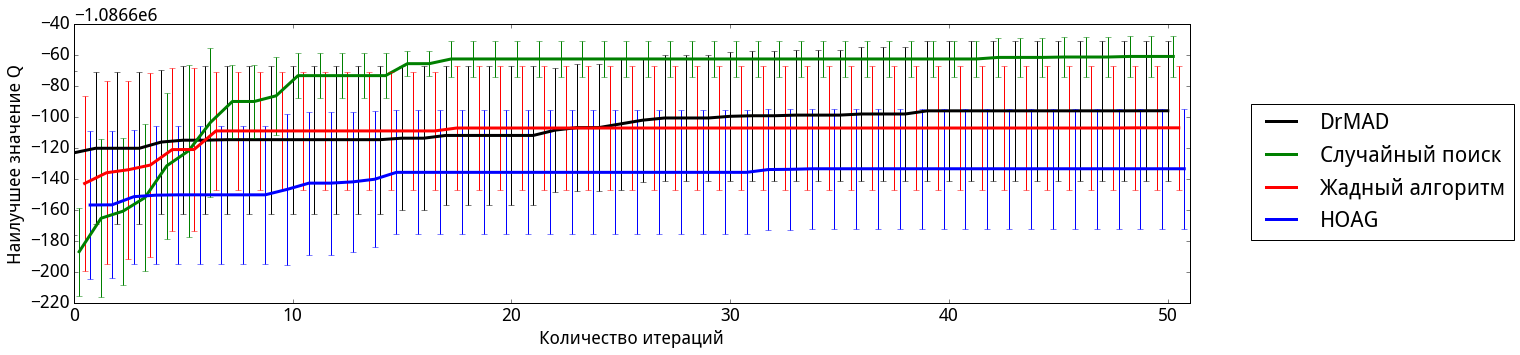
\includegraphics[width=\textwidth]{./slide_plots/wisdm_q_cv.png}
\end{figure}
\begin{figure}[h]
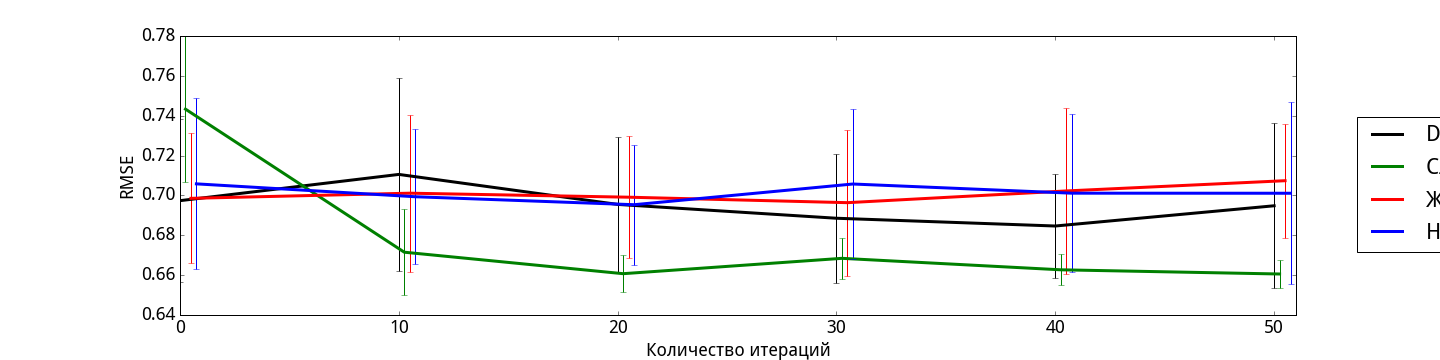
\includegraphics[width=\textwidth]{./slide_plots/wisdm_e_cv.png}
\end{figure}
\end{frame}

\begin{frame}{WISDM: вариационная оценка}
\begin{figure}[h]
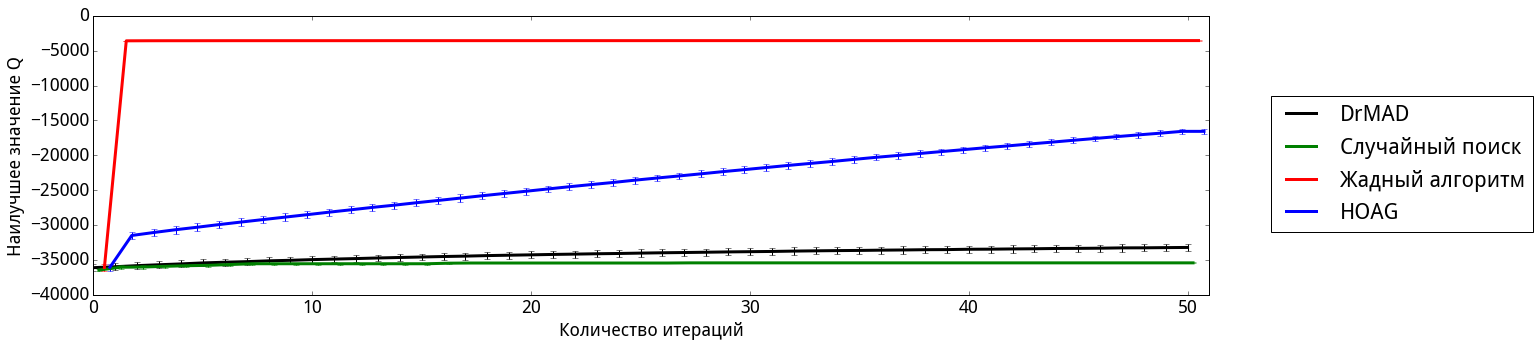
\includegraphics[width=\textwidth]{./slide_plots/wisdm_q_var.png}
\end{figure}
\begin{figure}[h]
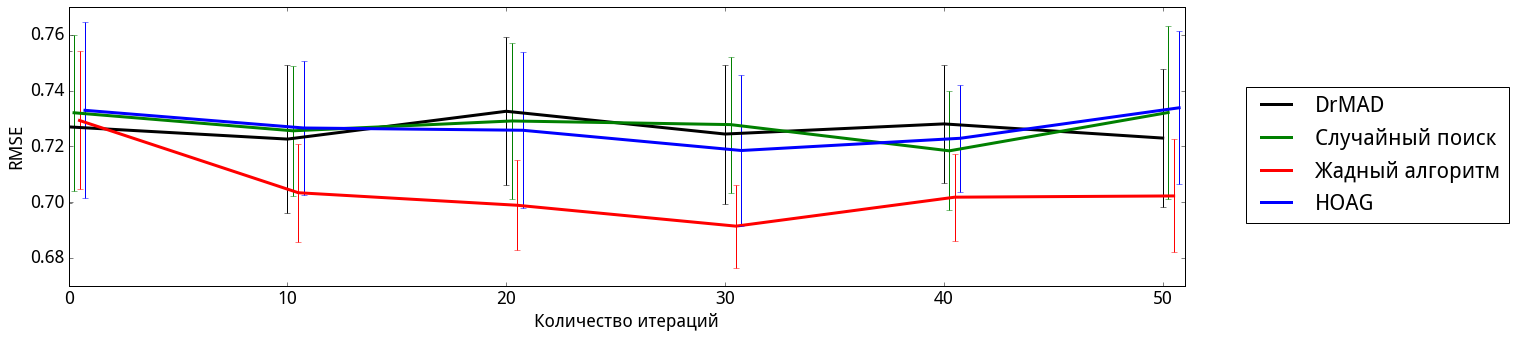
\includegraphics[width=\textwidth]{./slide_plots/wisdm_e_var.png}
\end{figure}
\end{frame}

\begin{frame}{MNIST: кросс-валидация}
\begin{figure}[h]
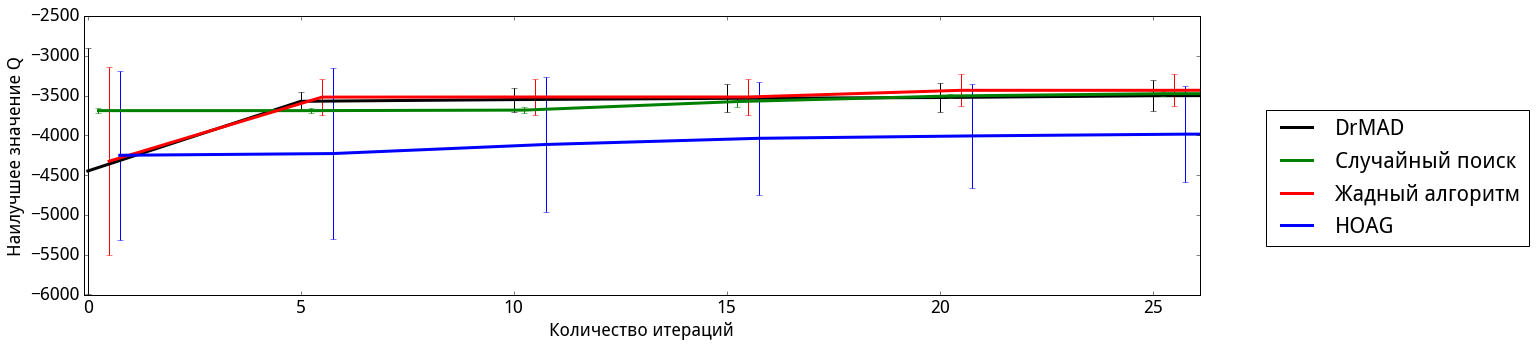
\includegraphics[width=\textwidth]{./slide_plots/mnist_q_cv.png}
\end{figure}
\begin{figure}[h]
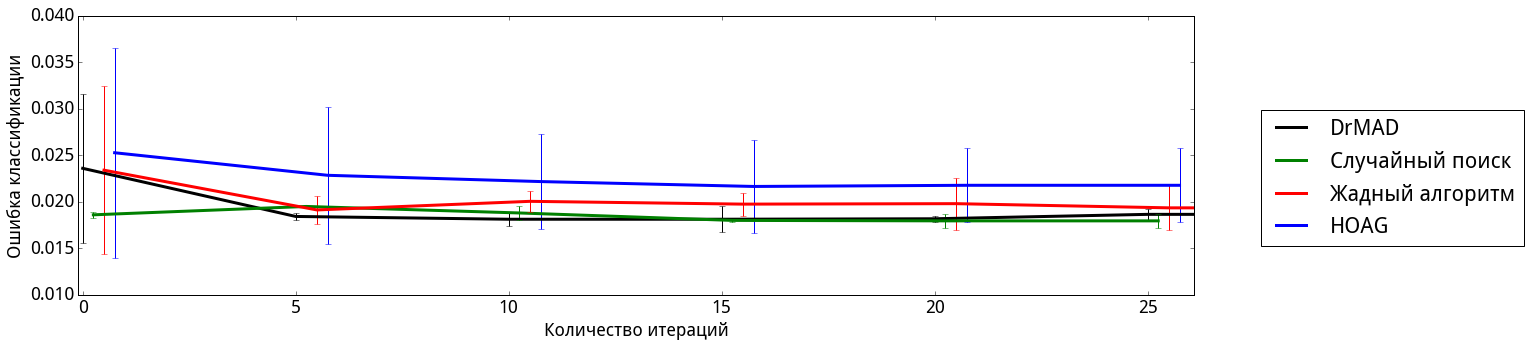
\includegraphics[width=\textwidth]{./slide_plots/mnist_e_cv.png}
\end{figure}
\end{frame}

\begin{frame}{MNIST: вариационная оценка}
\begin{figure}[h]
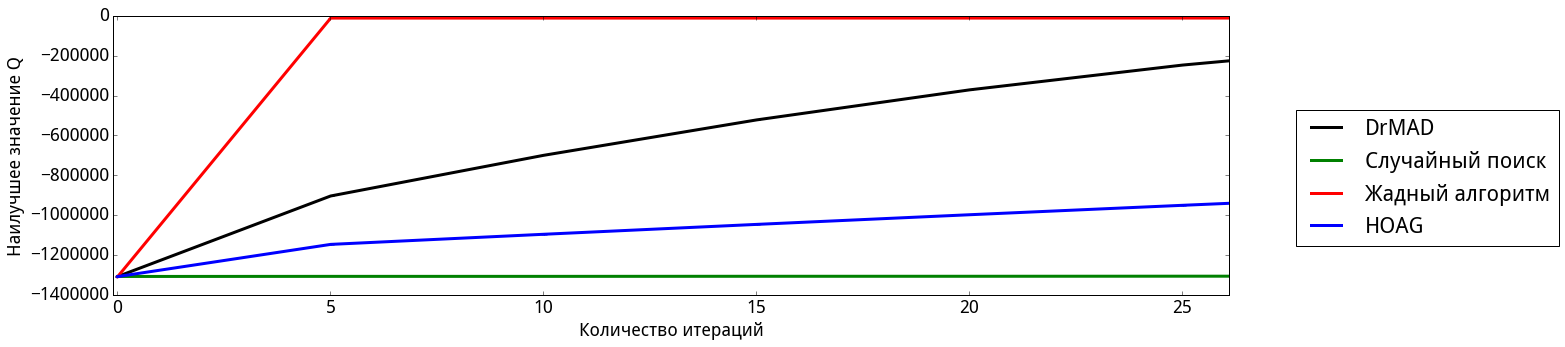
\includegraphics[width=\textwidth]{./slide_plots/mnist_q_var.png}
\end{figure}
\begin{figure}[h]
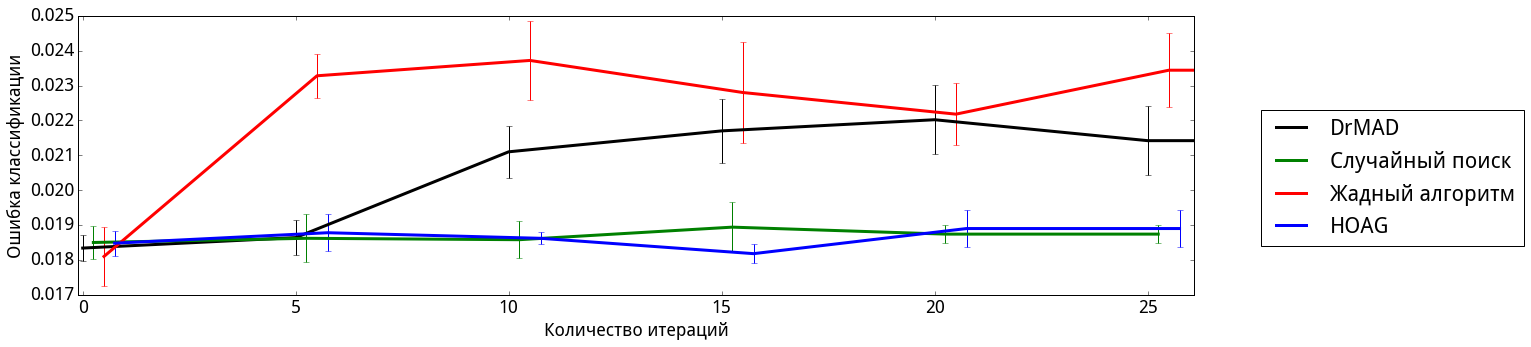
\includegraphics[width=\textwidth]{./slide_plots/mnist_e_var.png}
\end{figure}
\end{frame}


\begin{frame}{MNIST: добавление шума}
Добавление гауссового шума $\mathcal{N}(\mathbf{0},\sigma^2\mathbf{I})$:
\setlength{\columnsep}{10pt}
\begin{multicols}{4}
\begin{figure}[h]
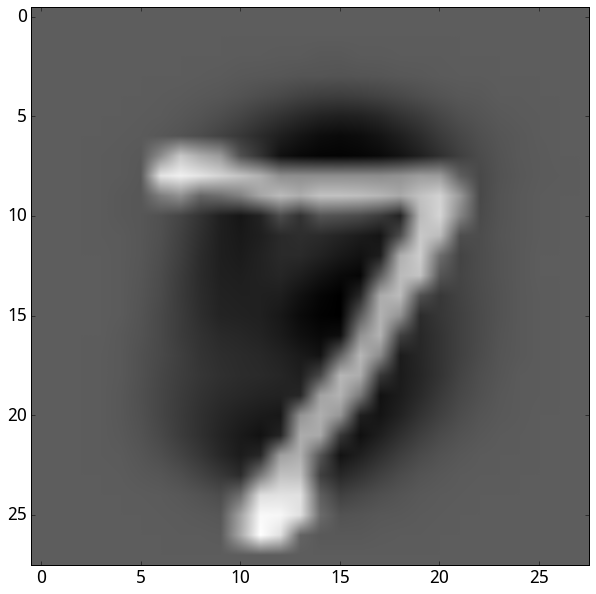
\includegraphics[width=0.10\textwidth]{./slide_plots/mnist0.png}
\caption*{Без шума}
\end{figure}

\begin{figure}[h]
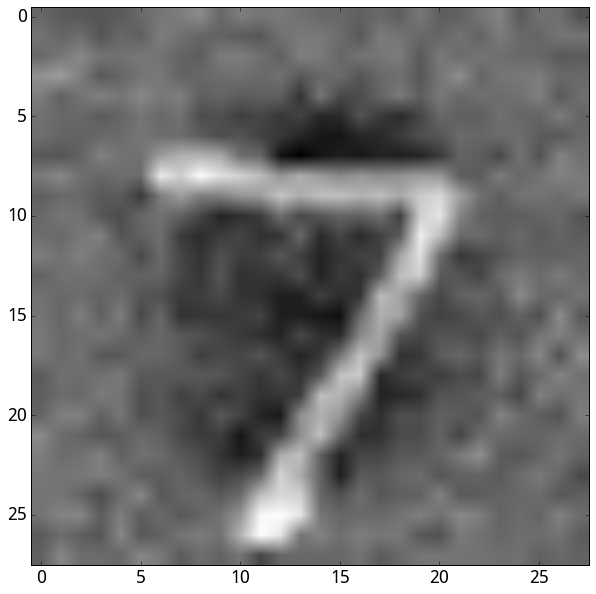
\includegraphics[width=0.10\textwidth]{./slide_plots/mnist10.png}
\caption*{$\sigma=0.1$}
\end{figure}

\begin{figure}[h]
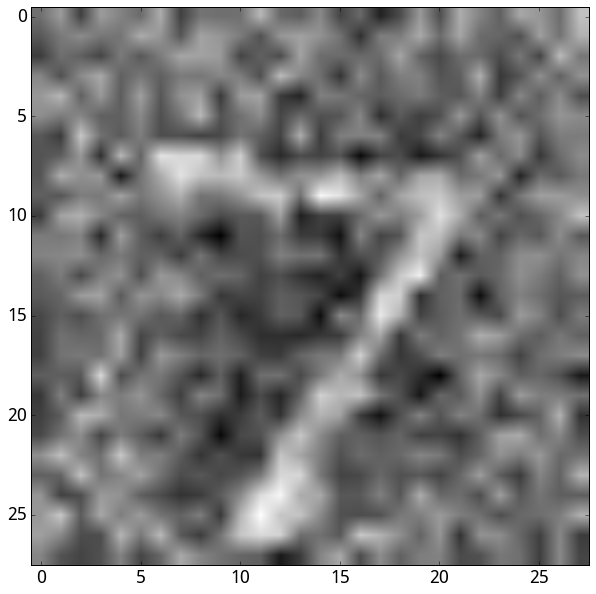
\includegraphics[width=0.10\textwidth]{./slide_plots/mnist25.png}
\caption*{$\sigma=0.25$}
\end{figure}

\begin{figure}[h]
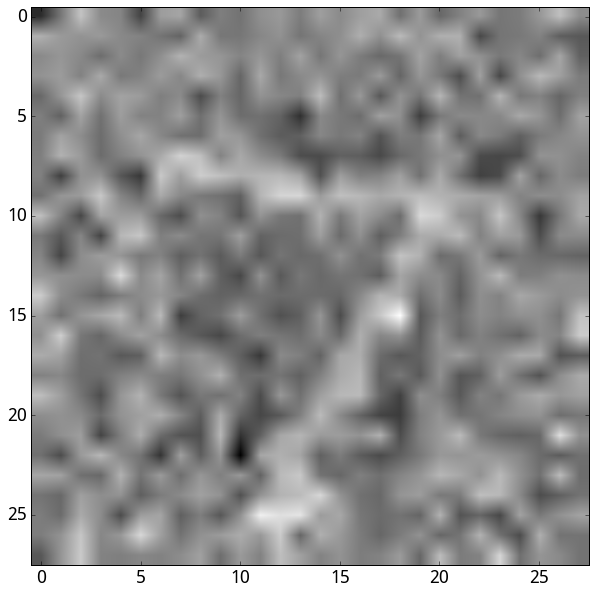
\includegraphics[width=0.10\textwidth]{./slide_plots/mnist50.png}
\caption*{$\sigma=0.5$}
\end{figure}
\end{multicols}
\begin{center}
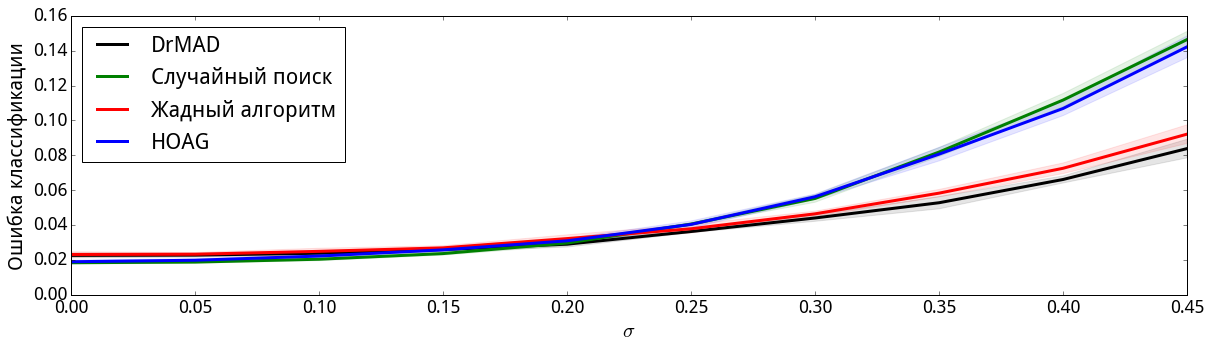
\includegraphics[width=0.9\textwidth]{./slide_plots/noise.png}
\end{center}
\end{frame}


\begin{frame}{Заключение}
\begin{itemize}
\item Предложен критерий оптимальной сложности модели глубокого обучения.
\item Исследована зависимость интегральной оценки правдоподобия от устойчивости модели и возможности переобучения.
\item Предложен алгоритм выбора субоптимальной модели классификации без использования кросс-валидации.
\item Рассмотрены градиентные алгоритмы оптимизации гиперпараметров.
\item Проведены эксперименты на ряде выборок в задачах классификации и регрессии.
\item Наилучшие результаты показали алгоритмы жадной оптимизации.
\end{itemize}
\end{frame}

\appendix
\bgroup
\setbeamercolor{background canvas}{bg=black}
\begin{frame}[plain, noframenumbering]
\end{frame}
\egroup



\begin{frame}[plain, noframenumbering]{Исследование основывается на следующих работах}
\begin{itemize}
\item Graves A. Practical variational inference for neural networks //Advances in Neural Information Processing Systems. – 2011
\item  Maclaurin D., Duvenaud D., Adams R. Gradient-based hyperparameter optimization through reversible learning //International Conference on Machine Learning. – 2015
\item  Luketina J. et al. Scalable gradient-based tuning of continuous regularization hyperparameters //International Conference on Machine Learning. - 2016
\item J. Fu et al., DrMAD: Distilling Reverse-Mode Automatic Differentiation for Optimizing
Hyperparameters of Deep Neural Networks // IJCAI - 2016
\item Pedregosa F. Hyperparameter optimization with approximate gradient //International Conference on Machine Learning. – 2016. –
\end{itemize}
\end{frame}


\end{document}
